\documentclass[conference]{IEEEtran}
%\documentclass[conference,letterpaper]{IEEEtran}
\IEEEoverridecommandlockouts
\usepackage[letterpaper, left=0.625in, right=0.625in, bottom=1in, top=0.75in]{geometry}
\usepackage[utf8]{inputenc} % input encoding for interpreter
\usepackage[T1]{fontenc}
%\usepackage{amssymb}
\usepackage{newtxtext}
\usepackage{multicol}
\usepackage{graphicx}
\usepackage[usenames,dvipsnames]{xcolor} % Allows the definition of hex colors
\usepackage{colortbl} % colors library.
\definecolor{klein}{HTML}{002fa7} % Klein blue
\usepackage[hyphens,spaces,obeyspaces]{url}
%\usepackage[colorlinks=True,citecolor=red,urlcolor=klein]{hyperref}% For Hyperlinks
\usepackage{cite}
\usepackage{amsmath,amssymb,amsfonts}
%\usepackage{algorithmic}
\usepackage{subcaption}
\usepackage{algpseudocode}
\graphicspath{ {./images/} }
\usepackage{textcomp}
\usepackage{xcolor}
\usepackage{makecell}
\usepackage[linesnumbered,ruled,norelsize]{algorithm2e}
\makeatletter
\newcommand{\removelatexerror}{\let\@latex@error\@gobble}
\makeatother
\usepackage{multicol}
\usepackage{mwe}
\newcommand\mycommfont[1]{\footnotesize\ttfamily\textcolor{blue}{#1}}
\SetCommentSty{mycommfont}

%\newcommand\mycommfont[1]{\footnotesize\ttfamily\textcolor{blue}{#1}}
%\SetCommentSty{mycommfont}
%
%\SetKwInput{KwInput}{Input}                % Set the Input
%\SetKwInput{KwOutput}{Output}              % set the Output

\def\BibTeX{{\rm B\kern-.05em{\sc i\kern-.025em b}\kern-.08em
   T\kern-.1667em\lower.7ex\hbox{E}\kern-.125emX}}

\begin{document}

\title{Energy-saving Cross-layer Optimization of Big Data Transfer Based on Historical Log Analysis\\
}

\author{\IEEEauthorblockN{Lavone Rodolph, MD S Q Zulkar Nine, Luigi Di Tacchio, and Tevfik Kosar} \IEEEauthorblockA{Department of Computer Science and Engineering, University at Buffalo, Buffalo, New York 14260, USA} \IEEEauthorblockA{
Email: \{lrodolph, mdsqzulk, luigidit,  tkosar\}@buffalo.edu}
}

\maketitle
\begin{abstract}
With the proliferation of data movement across the Internet, global data traffic per year has already exceeded the Zettabyte scale. The network infrastructure and end-systems facilitating the vast data movement consume an extensive amount of electricity, measured in terawatt-hours per year. This massive energy footprint costs the world economy billions of dollars partially due to energy consumed at the network end-systems. Although extensive research has been done on managing power consumption within the core networking infrastructure, there is little research on reducing the power consumption at the end-systems during active data transfers. This paper presents a novel cross-layer optimization framework, called Cross-LayerHLA, to minimize energy consumption at the end-systems by applying machine learning techniques to historical transfer logs and extracting the hidden relationships between different parameters affecting both the performance and resource utilization. %Data transfers rarely achieve the promised/advertised throughput/bandwidth promised/advertised by the lower layer network protocols due to poorly tuned data transfer parameters and computer resources. Prolonged computer resource usage increases end-system energy consumption. Heuristically tuning suboptimal data transfer parameters on line is an expensive task. Over estimating data transfer parameters and over provisioning compute resources can increase  energy cost. Under estimating data transfer parameters and under provisioning compute resources can reduce throughput performance. We can reduce online tuning by accurately estimating application layer data transfer parameters and kernel level parameters    by analyzing data transfer historical data logs utilizing machine learning techniques and mathematical analysis to find patterns. 
% It utilizes offline analysis to improve online learning approaches to optimally tune application-level and kernel-level parameters dynamically with minimal overhead.
It utilizes offline analysis to improve online learning and dynamic tuning of application-level and kernel-level parameters with minimal overhead. This approach minimizes end-system energy consumption and maximizes data transfer throughput. Our experimental results show that Cross-LayerHLA outperforms other state-of-the-art solutions in this area. 
%reducing energy consumption by 50\% and increasing data transfer throughput by 80\%.
\end{abstract}

\begin{IEEEkeywords}
energy-efficient data transfers, cross-layer optimization, dynamic parameter tuning, historical log analysis.
\end{IEEEkeywords}

%-------------------------------------------
\section{Introduction}
With the vast amount of data produced by scientific and engineering applications, social media, cloud computing, and the emerging Internet of Things (IoT), it is estimated that by 2022 the global Internet traffic will exceed 4.8 zettabytes per year caused by a projected 28.5 billion network-connected devices~\cite{CiscoWhitePaper2020}. 
%
The energy consumption of telecommunication networks has already exceeded 350 terawatt-hours, and the Internet comprises more than 10\% of the overall energy consumption in many countries, costing the global economy billions of dollars per year~\cite{GWATT}.
%
This massive energy footprint has ignited immense research in power-aware networking, focusing on reducing power consumption at both the hardware and systems-levels, including network devices.

A large portion of the existing energy-efficient networking research focuses on reducing power consumption within the core networking infrastructure (e.g., switches, hubs, and routers). State-of-the-art power-aware networking techniques include emerging architectures with programmable switches~\cite{greenberg2008towards}, power-aware networking protocols designed to consider energy consumption while routing data~\cite{chabarek2008power}, and putting idle components to sleep~\cite{gupta2003greening}. On the other hand, many of the existing core infrastructure solutions have shortcomings. For example, putting idle components to sleep can be detrimental to throughput. Also, replacing existing network switches and network protocols with power-aware switches and energy-efficient network protocols are expensive solutions and not practical in the short term. This paper presents a cost-effective, energy-efficient, practical end-system solution, called Cross-LayerHLA, which is an optimization framework that combines offline historical log analysis with dynamic online tuning to minimize end-system energy consumption and maximize data transfer throughput.

The major contributions of Cross-LayerHLA include: 
\begin{itemize}
    \item To the best of our knowledge, it is the first to integrate cross-layer adaptive online tuning with offline analysis using machine learning techniques to reduce energy consumption at the end systems and improve data transfer throughput performance.
    \item It is the first to dynamically tune both application-level and kernel-level data transfer parameters while obtaining optimal parameter values from offline analysis based on real-time network conditions.
    \item Compared to state-of-the-art solutions, it reduces end-system energy consumption during data transfers considerably while increasing the data transfer throughput at the same time.
\end{itemize}
 
The rest of this paper is organized as follows: Section \textrm{II} describes the related work in the field; 
%data transfer logs utilizing machine learning techniques; Section \textrm{III} describes how we model and optimize Service Level Agreements (SLAs) during the offline phase and use the corresponding algorithms during the online phase;  
Section \textrm{III} describes how we model and optimize energy consumption and throughput performance based on historical log analysis and dynamic online tuning;   Section \textrm{IV} evaluates Cross-LayerHLA and compares it to other state-of-the-art solutions in this area;  and Section \textrm{V} concludes the paper. 

%-----------------------------------------------------
\section{Related Work}

Prior work on application level tuning of transfer parameters mostly proposed static or non-scalable solutions to the problem with some predefined values for the subset of the problem space~\cite{R_Hacker02, R_Dinda05}. The main problem with such solutions is that they do not consider the dynamic nature of the network links and the background traffic in the intermediate nodes. 
%
Kasparan et al.~\cite{kaspar2010using} analyzed how pipelining affects throughput in local area networks and high-speed downlink packet access networks. 
%
Natarajan et al.~\cite{natarajan2009multiple} showed that using a single stream for transferring independent web objects is very inefficient in high latency networks. Using concurrent channels for delivering such objects increases download rates and decreases browser response times by enabling concurrent rendering. 
%
Robert et al.~\cite{kuschnig2010improving} used parallel file requests to increase usage of available bandwidth during Internet video streaming. 
%
Li et al.~\cite{liu2011parallel} presented a parallel streaming method instead of traditional adaptive sequential streaming. In distributed network environments, fetching media segments by parallel channels increases streaming performance and also copes with inefficient usage of resources.
%
Alan et al.~\cite{alan2015energy} analyzed the effects of different application-layer protocol parameters such as TCP pipelining, parallelism and concurrency levels on end-to-end throughput versus total energy consumption.

In our prior work~\cite{di2019cross}, we combined application-level (pipelining, parallelism, and concurrency) and kernel-level parameters (number of active cores, CPU frequency level) to minimize energy consumption at the end systems (source and destination nodes) during active data transfers. In that work, we heuristically performed the optimization without considering historical log analysis, but its convergence to optimal values was slow. In this work, we optimize data transfers and reduce energy consumption by jointly employing offline historical analysis, machine learning techniques, and online dynamic real-time tuning.

\section{Modeling and Optimizing Transfer Throughput and Energy Consumption}
To accurately model the data transfer throughput and end-system energy consumption, we consider and ensure that:
(1) our model is representative and characteristic of real-world data transfers; (2) our model accounts for fluctuating networking conditions, external background traffic, and external network loads; and (3) our model considers dataset characteristics (dataset size, average file size within a dataset, and file size distribution). The dataset characteristics would have a significant impact on transfer throughput performance and end-system energy consumption~\cite{alan2015energy}. For example, transferring a dataset comprised of multiple small files (such as text files) can benefit significantly from high concurrency and pipelining, and transferring a single large file would benefit from parallelism. To convey the impact of the kernel-level and application-level transfer parameters on end-system energy consumption and throughput performance, we express the relationships as the following functions:  
%$a_{bc}$
\begin{equation}
\label{Energy_Equation_2}
E = f_1(cpu_{num}, cpu_{freq}, cc, p, pp, data, net)\newline 
\end{equation}
\begin{equation}
\label{Throughput_Equation}
T = f_2(cpu_{num}, cpu_{freq}, cc, p, pp, data, net) 
\end{equation}
where $E$ is the energy consumption, $T$ is the throughput performance, $cpu_{num}$ is the number of active CPU cores, $cpu_{freq}$ is the frequency level of each active CPU core, $cc$ is the concurrency level, $p$ is the parallelism level, $pp$ is the pipelining level, $data$ is the dataset characteristics and $net$ is the network characteristics.

To address the factors above, we chose to: 
(1) accumulate and store real-world historical log data transfer information; %Each log entry contains data transfer meta-information corresponding to real-world data transfers.
(2) utilize machine learning to perform clustering on the historical log files, grouping/stratifying similar log entries based on network conditions, dataset meta-information, and network characteristics to uncover hidden relationships; and (3) derive an appropriate interpolation or regression model based on the rendered data characteristics. These steps are explained in the offline optimization subsection below.

%\section{Modeling and Optimizing SLA}
\subsection{Offline Analysis}

\textbf{Step 1: Accumulate and cache historical log data:}
During a data transfer, we accumulate the following information: i) throughput performance; ii) energy consumption; iii) network characteristics; iv) end-system resource usage; v) dataset characteristics; and vi) kernel-level and application-level parameter configuration.
Kernel-level and application-level parameter configuration includes: i) the number of active CPU cores; ii) the frequency level in which the active CPU cores operate; iii) concurrency; iv) parallelism; and v) pipelining. Historical log files are accumulated periodically and cached in a log server. 

\textbf{Step 2: Stratify historical log data:}
After accumulating historical log data, we stratify the log entries based on similar data characteristics. We utilize Hierarchical Agglomerative Clustering (HAC)~\cite{murtagh2014ward} with the Unweighted Pair Group Method with Arithmetic Mean (UPGMA)~\cite{gronau2007optimal} to achieve this. Also, we enforce artificial boundaries based on data transfers' distribution characteristics to ensure accurate stratification. Boundaries are based on the mean, and standard deviation of the achieved throughput and energy consumption of multiple collective data transfer runs. 
We utilize a bottom-up approach to cluster data in tiers. For tier 1, we cluster log entries based on external network characteristics. For tier 2, we apply agglomerative hierarchical clustering within each of the tier 1 clusters, further grouping log entries based on dataset meta-info (dataset size, file distribution, average file size and number of files in dataset). Since high external network loads decreases throughput performance and increases end-system energy consumption we further stratify the strata/data into interval ranges based on the data transfer logs' external network load distribution characteristics. This is necessary as current optimal parameters may become suboptimal as external network traffic changes. 
%during a data transfer, the current transfer parameters may not be optimal anymore and will need to be adjusted. The four interval ranges are: (1) minimum external network load  to  ( external network load mean $(extNet_\mu) - $ external network load standard deviation$(extNet_\sigma)$; (2) $(extNet_\mu - extNet_\sigma)$ to $extNet_\mu$; %$mean(\mu) - standard deviation (\sigma)$ 
%(3) $extNet_\mu$ to ($extNet_\mu + extNet_\sigma$); and (4) ($extNet_\mu + extNet_\sigma$) to max external network load. %This was necessary to maintain optimal parameters because the external network load may change throughout a data transfer rendering current transfer parameters non-optimal phasing out current  during a data transfer 
%Mean to standard deviation() 
For tier 3, we further group tier 2 clusters based on network characteristics such as source and destination nodes and their corresponding bandwidth and latency.

\iffalse
//Change Font
\begin{figure}[!t]
\begin{algorithm}[H]
  datasets = ClusterFiles() via Hierarchical Agglomerative Clustering\\
  \For{Timeout}
   {
     calculateDeltaEnergy()        \\
     calculateWeightedThroughput() \\
     calculateDeltaRtt().    \\
     t = dataSize/Tavg.    \\
     E_{pred} = P_{avg} * t      \\
     calculateExternalNetworkPercentage()\\
     
     \If{Ext_{Net} $>$(1 + \beta) * refExtNet}{
         \STATE $surface_{\theta} \leftarrow NewOptParams$
        }\Else { {Ext_{Net} $<$ (1 - \alpha) * ExtNet_{Last}} }
        
     
    \If{$\Delta$E_L_a_s_t$ $>$ (E_{pred} $x$  _{past}E_{pred} } 
       
        
    }
    pipelining = \lceil BDP $/$ avgFileSize \rceil \\
   }

   
  
\caption{Offline Non-Uniform Mixed Dataset Analysis/ Processing}
\end{algorithm}
\end{figure}
\fi

\iffalse
//Change Font
\begin{figure}[!t]
\begin{algorithm}[H]
  datasets = ClusterFiles() via Hierarchical Agglomerative Clustering\\
  \For{dataset in datasets}
   {
        \If{avgFileSize $>$ BDP}
    {
        dataset.splitFiles(BDP) \\
        
    }
    pipelining = \lceil BDP $/$ avgFileSize \rceil \\
   }
   tputChannel = avgWinSize $/$  RTT \\
   numChannels = \lceil bandwidth $/$ tputChannel \rceil \\
   \For{dataset in datasets}
   {
        weight_{i} = partitionSize_{i} $/$ \sum{partitionSize_{i}} \\
        concurrency = \lceil weight_{i} $x$ numChannels \rceil \\ 
   }
  \If{SLApolicy\{Energy\}}
    {
        numActiveCores = 1 \\
        CPUFrequency = minFrequency\\
    }
    \ElseIf{SLApolicy\{Throughput\}}
    {
     numActiveCores = maxCores \\
        CPUFrequency = minFrequency\\	
    }
\caption{Offline Non-Uniform Mixed Dataset Analysis/ Processing}
\end{algorithm}
\end{figure}
\fi

%Change Font

\textbf{Step 3: Derive interpolation/regression model:}
After data is accumulated, stratified, and categorized, we analyze and extract the hidden relationships within them. Since estimated energy consumption and throughput can be modeled as polynomial surfaces, we utilized piece-wise cubic spline interpolation ~\cite{ bickley1968piecewise} to derive the interpolants for each cluster/stratum. Second-order (quadratic) polynomial interpolation and third-order (cubic) polynomial interpolation based on Newton's or Lagrange's methods ~\cite{kincaid2009numerical} do not fit the data as smoothly as piece-wise cubic polynomials, which assures smoothness up to the second derivative. Since each data transfer parameter has distinct qualities, we model them independently. We first model a 2-dimensional cubic spline interpolation for energy consumption utilizing the number of CPU cores, denoted as cpu, as the abscissas and the end-system energy consumption values, denoted as e, as the ordinates. 

\begin{equation}
\label{Energy_Equation_1}
e_i = s_i(cpu_i) 
\end{equation} 

Given a cluster/stratum of discrete points which we will refer to as knots in a 2-dimensional space $\{(cpu_i,e_i)\}$, $i=1,...,N$, we formulate the interpolant $e_i = s(cpu_i)$ by using the piece-wise polynomial $s_i(cpu)$ as a nexus bridging together the pair of consecutive knots $(cpu_i,e_i)$ and $(cpu_{i+1},e_{i+1})$. This allows us to derive natural relaxed piece-wise cubic polynomials, where each $e_i$ have zero second derivatives at the end knots and assures curvature smoothness by restricting its coefficients. We can define each cubic polynomial piece as: 
\begin{IEEEeqnarray}{rCl} 
s_i(cpu_i)&=&a_{i,0}+a_{i,1}cpu+a_{i,2}cpu^2+ a_{i,3}cpu^3, \nonumber\\
&&
\forall cpu \in [cpu_i, cpu_{i+1}]
 \label{eq:new_cubicPieceWisePoly}
\end{IEEEeqnarray}

Since we have $N-1$ piece-wise cubic polynomials, we have $4(N-1)$ unknown coefficients $a_{i,j}$ where $j = 0,1,2,3$ of piece-wise cubic polynomial $s_i(cpu)$. We also have $N$ continuity conditions/stipulations for all given knots evaluated by the corresponding piece-wise cubic polynomial as specified by:

\begin{equation}
\label{condition_1}
s_i(cpu_i) = e_i, \quad i = 1,..,N \newline 
\end{equation} 
Furthermore, we have $N-2$ continuity conditions/stipulations for all interior knots specified as:
\begin{equation}
\label{condition_2}
s_i(cpu_{i+1}) = s_{i+1}(cpu_{i+1}), \quad i = 1,..,N-2 \newline
\end{equation} 

Utilizing Leibniz's notation for differentiation~\cite{thurston1973leibniz}, we can specify $N-2$ slope continuity conditions/stipulations for the interior knots as:
\begin{equation}
\label{condition_3}
\frac{ds_i}{d(cpu)} (cpu_{i+1}) =  \frac{ds_{i+1}}{d(cpu)} (cpu_{i+1}) \quad i = 1,..,N-2 \newline
\end{equation} 

This produces $N-2$ quadratic polynomial continuity stipulations. We also enforce $N-2$ additional continuity stipulations for the interior knots utilizing the second derivative as follows:  
\begin{equation}
\label{condition_4}
\frac{d^2s_i}{d^2(cpu)} (cpu_{i+1}) =  \frac{d^2s_{i+1}}{d^2(cpu)} (cpu_{i+1}) \quad i = 1,..,N-2 \newline
\end{equation} 
This produces $N-2$ Linear polynomial stipulations. Since we are constructing a natural relaxed piece-wise cubic spline polynomial the second derivative at the end knots are zero and may be specified as follows:
\begin{equation}
\label{condition_5}
\frac{d^2s}{d^2(cpu)} (cpu_1) =  \frac{d^2s}{d^2(cpu)} (cpu_n) = 0 \newline
\end{equation} 


By solving the system of linear equations we obtain the coefficients.\par 
End-system energy consumption also depends on the other four data transfer parameters: frequency (freq), concurrency (cc), pipelining (pp), and Parallelism (p). We extend the above example to formulate three multivariate piece-wise cubic spline polynomials corresponding to cubic polynomial surfaces. These include: $e_1=s(cpu,freq)$, $e_2=s(cc,p)$ and $e_3=s(pp)$. For each cubic spline polynomial we obtain the optimal parameter values based on data transfer service level agreements (SLA) and perform uniform sampling matching the criteria. 
%This is necessary as optimal transfer parameter values needed to meet a particular SLA may not be present in the historical log data. We selected the piece-wisecubic-spline surface interpolation method~\cite{kincaid2009numerical}, ~\cite{bickley1968piecewise}, ~\cite{walsh1962best},~\cite{ahlberg1963convergence},~\cite{sharma1966degree} as we observed the relationships between the data within clusters/strata were non-linear.  In addition, prior work revealed that both quadratic (second- order polynomial) regression and cubic (third-order) regression had a propensity to under-fit data ~\cite{nine2017bigData}. 
Utilizing piece-wise cubic-spline surface interpolation, we were able to stitch together multiple cubic functions and predict/estimate both energy consumption and throughput performance of the previously missing parameters. This was necessary as optimal transfer parameter values needed to meet a particular SLA may not be present in the historical log data. To test the accuracy of our cubic spline interpolation method, we used 70\% of the logs to perform the interpolation and the remaining 30\% as the test data. We used the standard Root Mean Squared Error (RMSE)~\cite{wiener1949wiener} to calculate the accuracy.  %This allows us to have a complete parameter space for each cluster and enables us to select the optimal transfer parameters for the given SLA. 

\iffalse
\begin{figure}[!t]
\begin{algorithm}[H]
{\scriptsize
  initializeParameters()\\
  \For{Timeout}
   {
       \If{instantaneous\_throughput \geq SLA}
    {
        \tcc{Uncongested period. Opportunity to advantageously augment throughput by increasing throughput
        constraint}
        advantageously\_augment\_constraint(SLA)\\
        \tcc{Obtain optimal parameters based on new SLA, offline analysis, current network load and data characteristics}
        
        getOptimalOffLineParameters(SLA,dataset,net,\delta)\\
    }\Else(instantaneous\_ throughput $<$ SLA){
    %\tcp{instantaneousThroughput < SLA}
        \If{under\_provisioned\_compute\_resources()}
        {
            \tcp{Low queuing delay detected}\\
            \tcp{}\\
            increase\_compute\_resources(SLA,dataset,net,\delta)\\
        }\Else(high queue delay detected){
            %\tcc*[h]{High Queue Delay Detected }\\
             enforceEqualStreamSharingPolicy()
        }
    }
}   
\caption{Dynamic Throughput Guarantee Tuning}
\end{algorithm}
\end{figure}
\fi

\iffalse
(See Engin's paper for wording on light external network load verses medium network load and high load)  our throughput algorithm we start with the optimal maximal parameters rendered from the polynomical surface tagged/labelled with the lightest external network load. This is in opposition to what Zulkar et al did, starting with the median load (then increasing or decreasing from there). We focus on core scaling, more so than frequency scaling. Also once the achieved throughput value gets outside the confidence interval or the achieved energy consumption is no longer within the confidence interval for this surface, either we obtain a lower external network polynomial surface  we apply heuristics. Note heuristics is only applied in throughput decreases below a certain specified threshold or if energy increases above a certain specified threshold. On Once we obtain optimal parameters we use heuristics to fine tune parameters. For mixed data transfers, we add or subtract channels from datasets based on the weight of the dataset. However, to maintain an optimal parameter ratio we do not recalculate and redistribute all channels based on the current weight like luigi did, but we add or subtract from the current channel distribution.  maintain channels based on the weight of  the number of concurrent channels based on the optimal channel to dataset ratio, and the weight of  current ratio of channels associated   Later with code, I can go between polynomial surfaces with different external network loads. In addition, we developed a new algorithm, energy per byte divides the energy interpolant by the throughput interpolant to obtain the minimum/most energy efficient/ minimum energy per byte per second. 
\fi
\subsection{SLA Optimization}
We developed two categories of service-level agreements (SLAs) as our optimization goals: (1) energy-constrained SLAs and (2) throughput assurance/guarantee SLAs. Based on the SLA type and the SLA specifications, we must select an optimal combination of the tunable parameters to satisfy the SLA requirements. To find the optimal parameter values for minimum end-system energy consumption, our energy-constrained optimization model determines the local minima in each of the three multivariate piece-wise cubic spline interpolation formulas and selects parameters corresponding to the minimum of the minima. This can be achieved by performing the second partial derivative test on all local minima, by calculating the Hessian matrix and determining if the matrix is positive definite. For throughput optimization, we perform the reverse, find all local maxima, calculate the Hessian matrix, and determine if the matrix is negative definite. We extend our previous optimization model ~\cite{nine2018greendataflow} to include kernel-level parameters and express it as:


\begin{equation}
\begin{aligned}
%& \min_{parameters,resources} \quad & (E) \\
& \min_{parameters(kernel,app)} \quad & (E) \\
& \qquad \textrm{subject to} \quad  &   T \geq T_{sla} 
\end{aligned}
\end{equation}

\begin{equation}
\begin{aligned}
& \max_{parameters(kernel,app)} \quad & \int_{T_s}^{T_f} T  \\
& \qquad \textrm{subject to} \quad & E \leq E_{sla} 
\end{aligned}
\end{equation}


The energy-constrained model allows a user to select optimal data transfer parameters that maximize throughput while ensuring the achieved energy consumption does not exceed the threshold specified by the SLA. The throughput guarantee model allows a user to select optimal data transfer parameters that minimizes energy consumption while ensuring the achieved throughput does not fall below the throughput threshold specified in the SLA. We utilize a Matlab solver to obtain optimal transfer parameters based on the specified SLA.

After the offline analysis is performed, we store optimized kernel-level and application-level transfer parameters %corresponding to the clusters’ throughput and energy SLA values 
in our custom data structure for our dynamic online program to use.  Each data structure instance corresponds to the optimal parameter configuration of a cluster satisfying the SLA.  
\iffalse
As previously discussed service providers and data center administrators already have an incentive/motivation to utilize/offer energy constrained SLA’s as energy-efficient data transfers can reduce the amount of energy expended at the end-systems/datacenter, thus reduce operational cost.   In addition, throughput guarantee services are also in demand as certain data transfers are throughput sensitive and are considered deadline-aware data transfers.
\fi

\iffalse %comment
\begin{figure}[!t]
\begin{algorithm}[H]
  datasets = partitionFiles()\\
  \For{dataset in datasets}
   {
        \If{avgFileSize $>$ BDP}
    {
        dataset.splitFiles(BDP) \\
        
    }
    pipelining = \lceil BDP $/$ avgFileSize \rceil \\
   }
   tputChannel = avgWinSize $/$  RTT \\
   numChannels = \lceil bandwidth $/$ tputChannel \rceil \\
   \For{dataset in datasets}
   {
        weight_{i} = partitionSize_{i} $/$ \sum{partitionSize_{i}} \\
        concurrency = \lceil weight_{i} $x$ numChannels \rceil \\ 
   }
  \If{SLApolicy\{Energy\}}
    {
        numActiveCores = 1 \\
        CPUFrequency = minFrequency\\
    }
    \ElseIf{SLApolicy\{Throughput\}}
    {
     numActiveCores = maxCores \\
        CPUFrequency = minFrequency\\	
    }
\caption{Heuristic parameter initialization ~\cite{di2019cross}}
\end{algorithm}
\end{figure}
\fi

\iffalse %COMMENT START
\begin{figure}[!t]
\begin{algorithm}[H]
  \For{timeout do}
   {
    calculateThroughput()\\
    measureQueuingDelay()\\
    measurePktLossRate()\\
    \For{dataset in datasets}
   {
    getPreComputedParameters(dataset,net\_status,\delta,SLA)\\
    }
   }
\caption{Slow Start Algorithm}
\end{algorithm}
\end{figure}
\fi %END COMMENT

\iffalse %START COMMENT
\subsection{Online Dynamic Tuning}
Before a data transfer starts, it's application-level and kernel-level tuning parameters are initialized based on heuristics considering current network conditions, dataset attributes and offline analysis
\fi %End Comment

\begin{figure}[!t]
%\begin{figure}[t]
\removelatexerror% Nullify \@latex@error
\begin{algorithm}[H]
\caption{Dynamic Energy Constraint Tuning}
  $datasets = ClusterFiles()$ \\
  \For{Timeout} {
     $calculateDeltaEnergy()$        \\
     $calculateWeightedThroughput()$ \\
     $calculateDeltaRtt()$    \\
     $t = dataSize / T_{avg}$    \\
     $E_{pred} = P_{avg} * t$      \\
     calculateExternalNetworkPercentage()\\
     startWithLightExtNetworkLoadSurface()\\
     \tcc{If Energy Increased}
     \If {$ (\Delta E_{last} + E_{pred} > (1+\beta) * pastE_{pred}) \parallel (\Delta E_{last} + E_{pred} > SLA) $} {
          \tcc{External Network Load Increased}
          \If{$ Ext_{Net} > (1 + \beta) * Ext_{ref_Net} $}{
                \tcc{Obtain Cluster/Surface with Higher External Network Load}
                $surface_{High\theta} \leftarrow NewOptParams$
          }
    }
          
    \tcp{Energy Decreased \& Ext Network Load Decreased}
    \ElseIf {$ refExtNet < (1 - \alpha) * Ext_{Net}_{Last} $}
    {
        $surface_{Low\theta} \leftarrow NewOptParams$
    }
}%End For
%\caption{Dynamic Energy Constraint Tuning}
\end{algorithm}
\end{figure}


\subsection{Online Dynamic Energy Constraint Tuning }

Cross-LayerHLA employs a dynamic online energy constraint tuning algorithm shown in Algorithm 1 derived from the offline energy constraint optimization model. Based on the energy constraint SLA, 
it periodically monitors the instantaneous power consumption at specified regular time intervals. If the instantaneous power consumption exceeds the threshold specified in the SLA, it obtains new optimal parameters within the confidence range/sampling region by obtaining a new energy polynomial surface that is closest to the current measured external network load and energy consumption range. If the measured instantaneous power consumption decreased from the last interval check, it obtains the closest energy polynomial surface and retrieves the associated optimal data transfer parameters. This is done approximately three times as continuously changing parameters are expensive.

\begin{figure}[!t]
\removelatexerror% Nullify \@latex@error
\begin{algorithm}[H]

  $datasets = ClusterFiles()$ \\
  \For{Timeout}
   {
     $calculateWeightedThroughput()$ \\
     $calculateDeltaRtt()$   \\
     $calculateExternalNetworkPercentage()$\\
     $startWithLightExtNetworkLoadSurface()$\\
     \tcc{If Throughput Decreased}
     \If { $T_{avg} < (1-\alpha) * T_{Last} \parallel (T_{avg} < SLA) $  } {\\
          \tcc{External Network Load Increased}
        \If{$Ext_{Net} > (1 + \beta) * refExtNet$}{
        \tcc{Obtain Cluster/Surface with Higher External Network Load}
         $surface_{High\theta} \leftarrow NewOptParams$
        }
     }%End the ELSE External Network Load 
    \Else { 
        \tcp{Throughput Increased}
        \If{
            \tcp{External Network Load decreased}
            $refExtNet < (1 - \alpha) * Ext_{Net}_{Last}$
           } {\tcc{Obtain Cluster/Surface with Lower External Network Load}
           $surface_{Low\theta} \leftarrow NewOptParams$}
    }
}%end For 
\caption{Dynamic Throughput Tuning}
\end{algorithm}
\end{figure}


\iffalse
advantageously decreases energy constraints to further reduce energy consumption(lines 3 - 4). During this low network congestion period, Cross-layerHLA obtains new optimal parameters based on the updated SLA constraints, current network conditions, dataset characteristics and offline analysis (line 5). 
However, if cross-layerHLA determines instantaneous power consumption surpassed the SLA specified threshold, it determines if the energy spike was caused by over-provisioning compute resources (low queue delay), high queue delay or high packet loss.  If the energy spike was due to over-provisioning compute resources, cross-layerHLA will obtain new optimal compute resources %(needed to optimaly continue the data transfer) 
from the online optimization module based on the SLA, current network conditions and data characteristics. If the energy spike was due to high queue delay indicating network congestion, cross-layerHLA will reduce parallelism (the number of parallel TCP streams) by a factor of $\alpha$. The action is encapsulated in the enforceEqualStreamSharingPolicy method  (line 12). If the energy spike was due to packet loss, indicating high network congestion, possibly caused by excessive packet re-transmissions %by TCP,
cross-layerHLA will reduce concurrency (the number of concurrent TCP streams) by a factor of $\beta$. The action is encapsulated in the enforceEqualStreamSharingPolicy method  (line 12)\par
\fi

\iffalse
\begin{figure*}[t]
    \begin{centering}
	\begin{subfigure}[t]{0.31\textwidth}
    	\centering
    	\caption{Chameleon Throughput (Mbps)}
        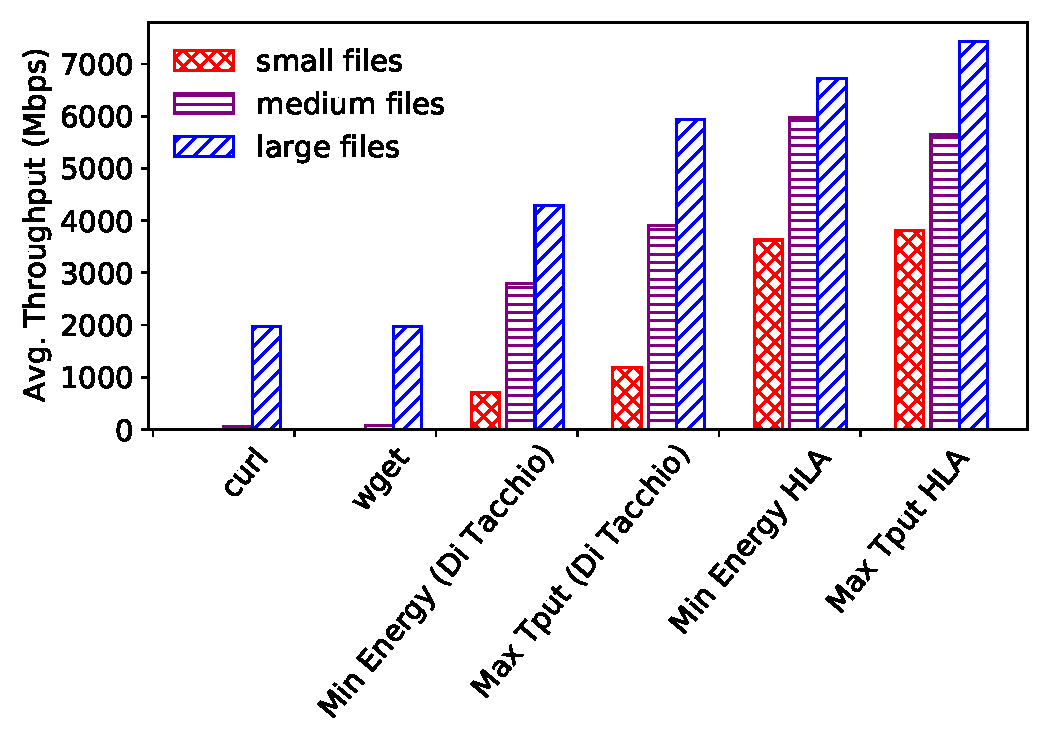
\includegraphics[keepaspectratio=true,width=58mm]{images/Chameleon_Client_Throughput_March_14FontSize.pdf}
        
        \vspace{-2mm}
        %\caption{Chameleon Throughput (Mbps)}
    \end{subfigure}
    \begin{subfigure}[t]{0.31\linewidth}
    	\centering
    	\caption{CloudLab Throughput (Mbps)}
        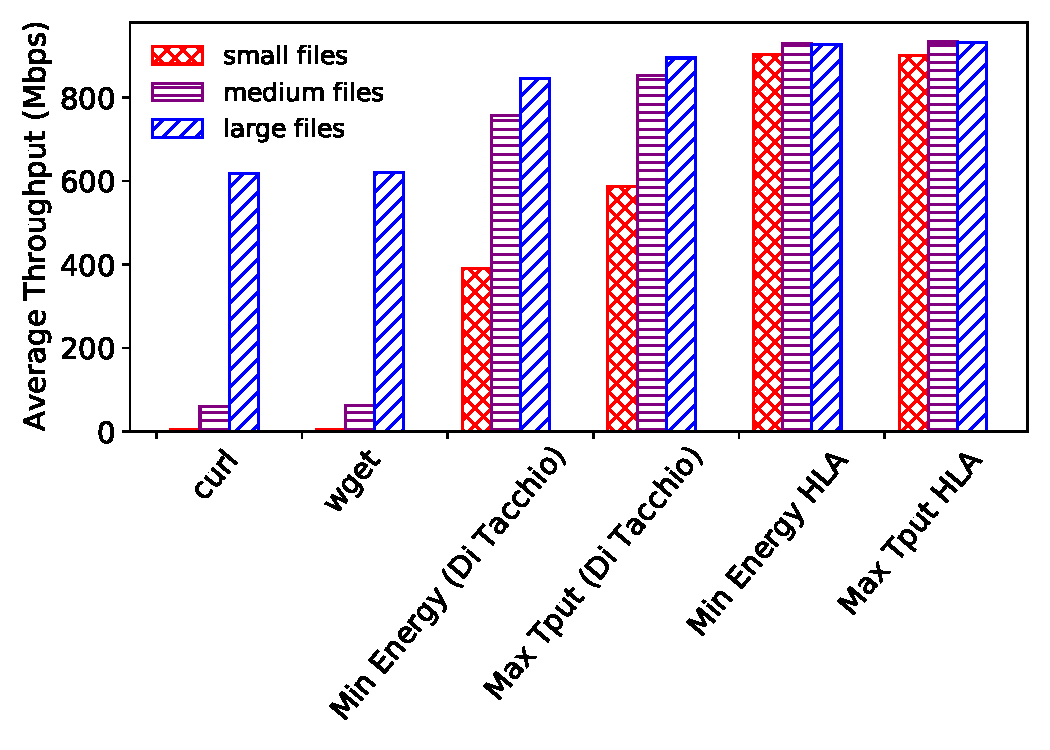
\includegraphics[keepaspectratio=true,width=58mm]{images/CloudLab_Client_Throughput_March_14FontSize.pdf}
        %\hspace{-20mm}
        \vspace{-2mm}
        %\caption{CloudLab Throughput (Mbps)}
    \end{subfigure}
    \begin{subfigure}[t]{0.31\textwidth}
    	\centering
    	\caption{Inter-Cloud Throughput (Mbps)}
        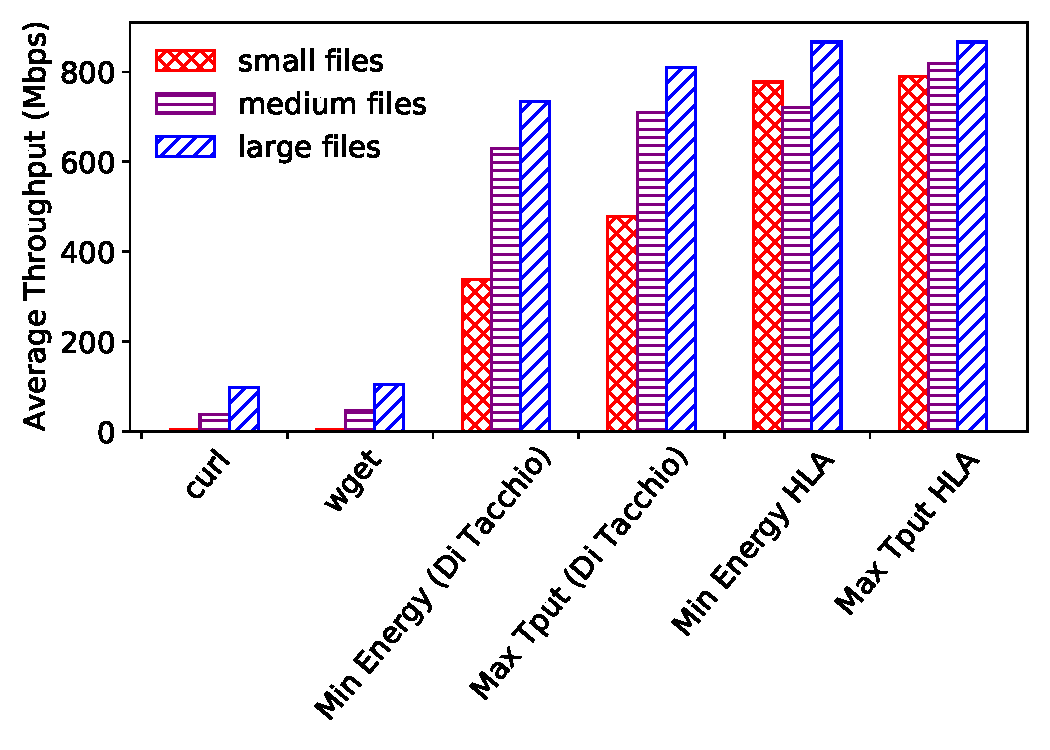
\includegraphics[keepaspectratio=true,width=58mm]{images/InterCloud_Client_Throughput_March_14FontSize.pdf}
        \vspace{-2mm}
        %\caption{Inter-Cloud Throughput (Mbps)}
    \end{subfigure}
	\begin{subfigure}[t]{0.31\textwidth}
    	\centering
    	\caption{Chameleon Client Energy (Joules)}
        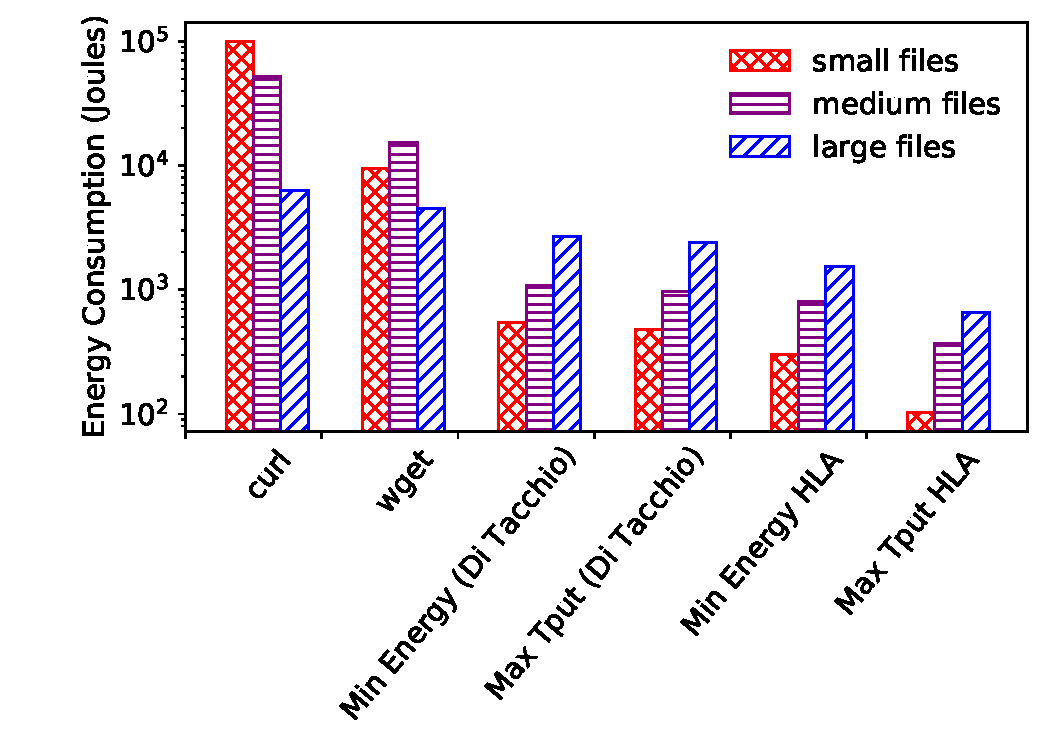
\includegraphics[keepaspectratio=true,width=58mm]{images/Chameleon_Client_Data_Transfer_Energy_March_14FontSize.pdf}
        \vspace{-2mm}
        %\caption{Chameleon Client Energy (Joules)}
    \end{subfigure}
 	\begin{subfigure}[t]{0.31\textwidth}
    	\centering
    	\caption{CloudLab Client Energy (Joules) }
        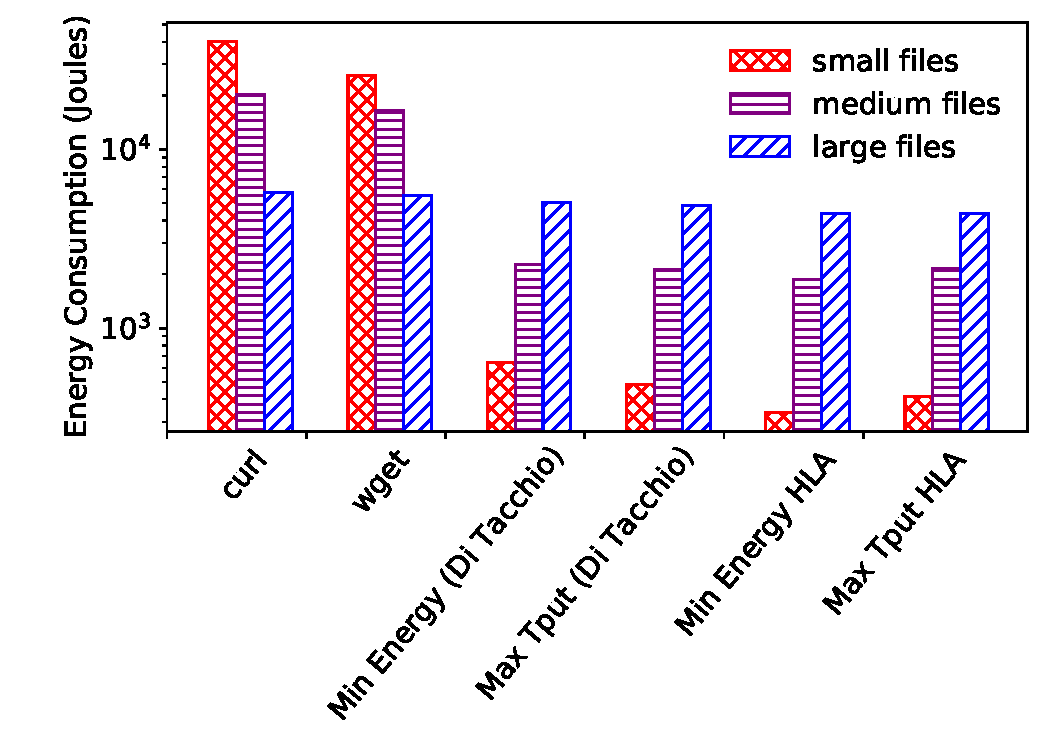
\includegraphics[keepaspectratio=true,width=58mm]{images/CloudLab_Client_Data_Transfer_Energy_March_14FontSize.pdf}
        \vspace{-2mm}
        %\caption{CloudLab Energy (Joules) }
    \end{subfigure}
    \begin{subfigure}[t]{0.31\textwidth}
    	\centering
    	\caption{Inter-Cloud Client Energy (Joules)}
        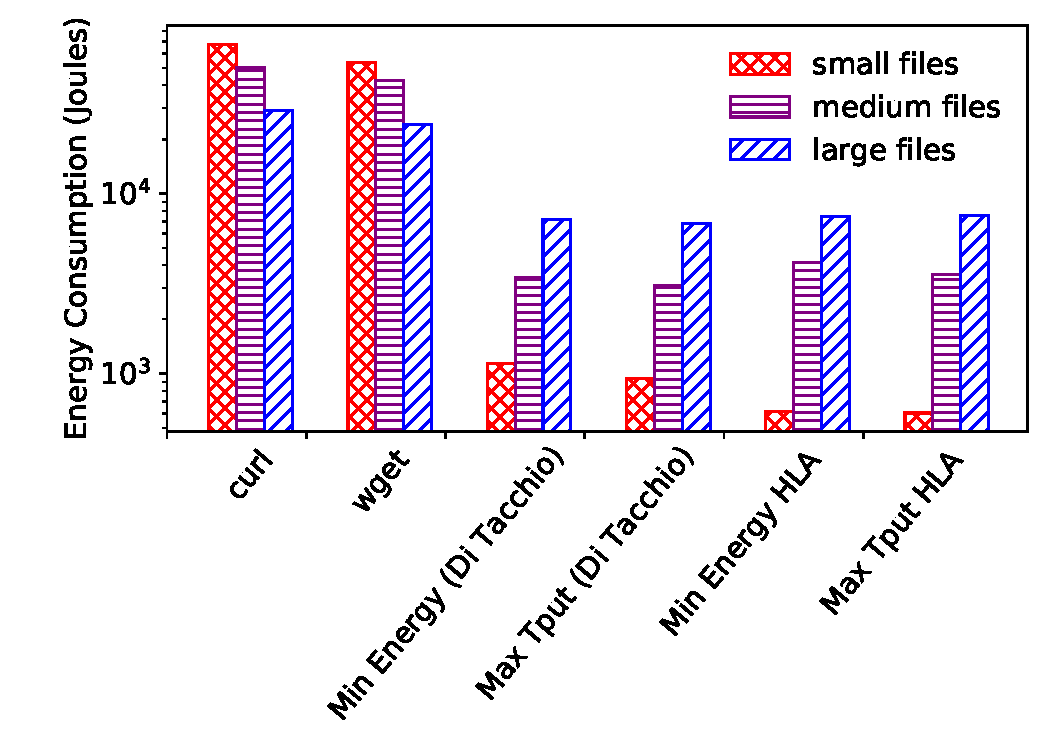
\includegraphics[keepaspectratio=true,width=58mm]{images/Inter-Cloud_Client_TotalEnergy_March_14FontSize.pdf}
        \vspace{-2mm}
        %\caption{Inter-Cloud Client Energy (Joules)}
    \end{subfigure}
     \caption{Achieved throughput (Mbps) and energy consumption (Joules) over 3 diverse testbeds}
     \vspace{-4mm}
     \label{fig:throughputresults}
     \end{centering}
 \end{figure*}
 \fi

\subsection{Online Dynamic Throughput Guarantee Constraint Tuning }
Cross-LayerHLA employs a dynamic online throughput constraint tuning algorithm shown in Algorithm 2 derived from the offline throughput constraint optimization model. In this algorithm, it periodically monitors the instantaneous throughput at specified regular time intervals. If the instantaneous throughput falls below the threshold specified in the SLA, it obtains new optimal parameters within the confidence range/sampling region by obtaining a new polynomial throughput surface that is closest to the current measured external network load. If the measured instantaneous throughput increased or decreased from the last interval check, it obtains the closest throughput polynomial surface and retrieves the associated optimal data transfer parameters for the associated external network load. Obtaining optimal parameters from the polynomial throughput surfaces is done at a maximum of three times since it is expensive to modify the data transfer parameters. Afterward, if necessary, data transfer parameters are adjusted heuristically.


\subsection{Testing Online Dynamic Algorithms }
In order to fairly compare the efficiency of our dynamic energy constraint algorithm and throughput guarantee algorithm with other transfer tools/solutions, we utilize the extreme use cases. To achieve this, we use an SLA policy that informs our dynamic energy constraint algorithm to transfer data with the least amount of energy/power consumption by utilizing joint optimal kernel-level and application-level parameters. We call this SLA policy the minimum energy consumption SLA. To test our throughput guarantee algorithm, we use an SLA policy that enforces our algorithm to transfer data with the maximum throughput rate achievable, utilizing joint optimal kernel-level and application-level parameters.


\iffalse
Cross-layerHLA periodically monitors the instantaneous throughput. If the instantaneous throughput exceeds/surpasses the SLA threshold, %cross-layerHLA determines there is low network congestion and will
cross-layerHLA advantageously increases the throughput constraints to further augment throughput (lines 3 - 4). Cross-layerHLA obtains new optimal parameters based on the updated SLA constraints, current network conditions, dataset characteristics an offline analysis (line 5). 
However, if %cross-layerHLA determines 
the instantaneous throughput falls below the specified SLA threshold, cross-layerHLA determines if the throughput drop was caused by under-provisioning compute resources (low queue delay), high queue delay or high packet loss.  If the throughput drop was due to under-provisioning compute resources, cross-layerHLA will obtain  optimal compute resources %(needed to optimaly continue the data transfer) 
from the pre-computed mathematical optimization module based on the SLA, current network conditions and data characteristics. If the throughput drop was due to high queue delay indicating network congestion, cross-layerHLA will reduce parallelism (the number of parallel TCP streams) by a factor of $\alpha$. The action is encapsulated in the enforceEqualStreamSharingPolicy method  (line 12). If the throughput drop was due to packet loss, indicating high network congestion, possibly caused by excessive packet re-transmissions %by TCP,
cross-layerHLA will reduce concurrency (the number of concurrent TCP streams) by a factor of $\beta$. The action is encapsulated in the enforceEqualStreamSharingPolicy method  (line 12).\par
In addition to comparing our dynamic energy constraint algorithm we also compare our dynamic throughput guarantee algorithm with other solutions. The objective of this SLA policy is to transfer data with the highest achievable throughput.   
We enforce this SLA policy by employing our dynamic throughput guarantee algorithm which periodically selects the optimal application-level and kernel-level tuning parameters based on the current network conditions, CPU resource usage and our offline analysis.
\fi

\iffalse %COMMENT
%PACKET LOSS INFO FROM Zulkars archived draft of GreenDataFlow
Challenge 2. (Packet loss) Any packet loss can reduce the TCP window size (cwnd) significantly (depending on the TCP variant) which reduces the achievable transfer throughput. Packet loss can happen for a range of reasons, such as: (1) congestion, (2) bottleneck network devices with low capacity (routers/switch/middleboxes), (3) software bugs in network devices, and (4) faulty links. We need a mechanism to detect the static packet losses (2-4) and eliminate them manually. We also need a mechanism that can efficiently signal congestion beforehand to avoid the TCP window size reduction.
\fi %End Data Flow

 \iffalse
 %Di Tacchio et al. initialization method specified in algorithm 1. We utilize this method because when a transfer starts we do not know the current network conditions and we need to do real time online probing before we can obtain optimal parameters from offline analysis.  When a data transfer task start, it starts in the slow start state. In this state the program gauges the network conditions and after a short specified period of time (delta) it selects the optimal values for the parameters based on offline analysis. Initially, in slow state, both the application-layer and kernel-layer parameters are initialized based on theoretical values rendered by the initialization algorithms. After the slow state period ends, the data transfer enters the steady state, in this state, the program periodically checks the network conditions and based on network condition changes and  SLA type makes application layer and kernel layer parameter adjustments.  If in steady state, the program determines that either the instantaneous throughput decreased below the specified throughput SLA or that instantaneous power consumption increased above the provided energy SLA, the program  adjust transfer parameters based on the assumed cause of the problem.  If the network condition change was due to congestion, the program determines if this was caused by a high queuing delay or by a high packet loss rate. In both cases TCP enacts it’s retransmission functionality which causes the congestion.  
\fi



\iffalse %COMMENT
\begin{figure}[!t]
\begin{algorithm}[H]
  initializeParameters()\\
  slowStart()\\
  \For{Timeout}
   {
       \If{state = STEADY}
    {
       \If{instPower $>$ SLA}{
         \If{highQueueDelay()}{
            decreaseParallelChannels()\\
         }
         \ElseIf{highPacketLoss()}{
         decreaseConcurrentChannels()
         }
         \tcc{OVER PROVISIONED COMPUTE RESOURCES }
         %\tcc{need NEW OPTIMAL (APPLICATION-LEVEL and KERNEL-LEVEL) PARAMETERS based on current network load, data characteristics, SLA and offline analysis}
         
         \Else{
         getUpdatedParameters(dataset,net\_status,\delta,SLA))\\
         }
         \tcc{Transition to the WARNING state}
         state = WARNING\\  
       }
       
    }
    \ElseIf{state = WARNING}
    {
       \If{instPower $>$ SLA}{
       updateSLAGoal()\\
       getUpdatedParameters(dataset,net\_status,\delta,SLA))\\
       }
       \Else{
         state = STEADY  \\   
         }
        
    }
    \\
   }
\caption{Dynamic Energy Constraint Tuning}
\end{algorithm}
\end{figure}
\fi %END Comment


 
\iffalse %START COMMENT **********
However, if high queuing delay was the cause, then the level of parallelism is reduced by a factor of alpha and the data transfer task enters the warning state. Please note, high queuing delay is recognized/determined when the current measured queuing delay goes beyond the specified threshold determined by many experimental runs/logs/trials.  If,  high packet loss rate is determined as the cause of congestion, then the level of concurrency is reduced by a factor of alpha, since the impact of packet loss rate is more severe than high queuing delay. The program then enters the warning state.  However, if  the steady state determined that the throughput drop for a throughput based SLA was caused by under-provisioning of resources (such as compute resources) than the program increases the number of active cores by beta based on the current CPU load or it increase the frequency level of the current active cores if the active number of CPU cores cannot be increased. The program then transitions to the warning state. If  the steady state determined that the energy spike for energy based SLA’s was caused by over-provisioning of resources (such as computer resources) than the number of active cores are scaled back by a factor of beta based on the current CPU load or the frequency levels are scaled down for all active cores, if the active number of cores cannot be reduced.  While in the warning state, when the program checks the network’s condition again, it obtains the optimal application-layer and kernel layer pre-computed parameters from the hash table based on off-line analysis corresponding to the current network condition (external network load) and proceeds back to the steady state, regardless of the SLA type. Figure X and Figure Y shows the finite state machine for both SLA types. Dynamic Throughput Algorithm 1 and Dynamic Energy Algorithm shows/illustrates/demonstrates the throughput based SLA algorithm and the energy based SLA algorithm respectfully.



\fi %END COMMENT ****************



\iffalse %Comment
\begin{figure}[!t]
\begin{algorithm}[H]
  initializeParameters()\\
  slowStart()\\
  \For{Timeout}
   {
       \If{state = STEADY}
    {
       \If{instThroughput $<$ SLA}{
         \If{highQueueDelay()}{
            decreaseParallelChannels()\\
         }
         \ElseIf{highPacketLoss()}{
         decreaseConcurrentChannels()
         }
         \tcc{Underprovisioned computing resources, need new parameters}
         \Else{
         getUpdatedParameters(dataset,net\_status,\delta,SLA))\\
         }
         
       }
    \tcc{Transition to the WARNING state}
         state = WARNING\\     
    }
    \ElseIf{state = WARNING}
    {
       \If{instThroughput $<$ SLA}{
       updateSLAGoal()\\
       getUpdatedParameters(dataset,net\_status,\delta,SLA))\\
       }
       \Else{
         state = STEADY  \\   
         }
        
    }
    \\
   }
\caption{Dynamic Throughput Guarantee Tuning}
\end{algorithm}
\end{figure}
\fi %END Comment

\iffalse
%\begin{figure*}[!t]%
\begin{figure*}%
%\centering
\begin{subfigure}{.65\columnwidth}

\includegraphics[width=\columnwidth]{cloudlab_tput}%
\caption{cap a}%
\label{subfiga}%
\end{subfigure}\hfill%
\begin{subfigure}{.65\columnwidth}

\includegraphics[width=\columnwidth]{cloudlab_tput.pdf}%
\caption{cap b}%
\label{subfigb}%
\end{subfigure}\hfill%
\begin{subfigure}{.65\columnwidth}

\includegraphics[width=\columnwidth]{cloudlab_tput.pdf}%
\caption{cap c}%
\label{subfigc}%
\end{subfigure}%
\newline
\begin{subfigure}{.65\columnwidth}

\includegraphics[width=\columnwidth]{cloudlab_tput.pdf}%
\caption{cap d}%
\label{subfigd}%
\end{subfigure}%
\begin{subfigure}{.65\columnwidth}

\includegraphics[width=\columnwidth]{cloudlab_tput.pdf}%
\caption{cap e}%
\label{subfige}%
\end{subfigure}%
\begin{subfigure}{.65\columnwidth}

\includegraphics[width=\columnwidth]{cloudlab_tput.pdf}%
\caption{cap f}%
\label{subfigf}%
\end{subfigure}%
\caption{The proper caption}
\label{figabc}
\end{figure*}
\fi


\iffalse
%\begin{figure*}[!t]%
\begin{figure*}%
%\centering
\begin{subfigure}{.65\columnwidth}

\includegraphics[keepaspectratio=true,width=\columnwidth]{cloudlab_tput}%
\caption{Energy Consumption (Chameleon Cloud)}%
\label{subfiga}%
\end{subfigure}\hfill%
\begin{subfigure}{.65\columnwidth}

\includegraphics[keepaspectratio=true,width=\columnwidth]{cloudlab_tput.pdf}%
\caption{cap b}%
\label{subfigb}%
\end{subfigure}\hfill%
\begin{subfigure}{.65\columnwidth}

\includegraphics[keepaspectratio=true,width=\columnwidth]{cloudlab_tput.pdf}%
\caption{cap c}%
\label{subfigc}%
\end{subfigure}%
\newline
\begin{subfigure}{.65\columnwidth}

\includegraphics[keepaspectratio=true,width=\columnwidth]{cloudlab_tput.pdf}%
\caption{cap d}%
\label{subfigd}%
\end{subfigure}%
\begin{subfigure}{.65\columnwidth}

\includegraphics[keepaspectratio=true,width=\columnwidth]{cloudlab_tput.pdf}%
\caption{cap e}%
\label{subfige}%
\end{subfigure}%
\begin{subfigure}{.65\columnwidth}

\includegraphics[keepaspectratio=true,width=\columnwidth]{cloudlab_tput.pdf}%
\caption{cap f}%
\label{subfigf}%
\end{subfigure}%
\caption{The proper caption}
\label{figabc}
\end{figure*}
\fi



\iffalse
\begin{figure*}[t]
    \begin{centering}
	\begin{subfigure}[t]{0.3\textwidth}
    	%\centering
        
\includegraphics[keepaspectratio=true,width=50mm]{cloudlab_tput}
        %\vspace{-2mm}
        
        \caption{Energy consumption (Chameleon Cloud)}
    \end{subfigure}
    \begin{subfigure}[t]{0.3\textwidth}
    	%\centering
        
\includegraphics[keepaspectratio=true,width=50mm]{cloudlab_tput}
        %\vspace{-2mm}
        \caption{Energy consumption (Cloud Lab)}
    \end{subfigure}
    \begin{subfigure}[t]{0.3\textwidth}
    	%\centering
        
\includegraphics[keepaspectratio=true,width=50mm]{cloudlab_tput}
        %\vspace{-2mm}
        \caption{Energy Consumption (Inter-cloud)}
    \end{subfigure}
	\begin{subfigure}[t]{0.3\textwidth}
    	%\centering
    	
\includegraphics[keepaspectratio=true,width=50mm]{cloudlab_tput}
        %\vspace{-2mm}
        \caption{Average Throughput (Chameleon Cloud)}
    \end{subfigure}
 	\begin{subfigure}[t]{0.3\textwidth}
    	%\centering
    	
\includegraphics[keepaspectratio=true,width=50mm]{cloudlab_tput}
        %\vspace{-2mm}
        \caption{Average Throughput (Cloud Lab)}
    \end{subfigure}
    \begin{subfigure}[t]{0.3\textwidth}
    	%\centering
        
\includegraphics[keepaspectratio=true,width=50mm]{cloudlab_tput}
        %\vspace{-2mm}
        \caption{Average Throughput (Inter-Cloud)}
    \end{subfigure}
     \caption{Comparison of throughput and energy consumption across 3 different testbeds}
     \vspace{-4mm}
     \label{fig:throughputresults}
     \end{centering}
 \end{figure*}
 \fi


 
\iffalse %COMMENT START ********************
\subsection{Minimum Energy Consumption SLA}
In order to fairly compare the efficiency of our dynamic energy constraint algorithm with other transfer tools/solutions as explained in our experimental evaluation results section we  compare/utilize the extreme use case. We set the SLA policy to transfer data with the least amount of energy/power consumption. We call this SLA policy the minimum energy consumption SLA. 
We enforce the minimum energy SLA policy by employing our dynamic energy constraint algorithm which periodically selects the optimal application-level and kernel-level tuning parameters based on the current network conditions, CPU resource usage, dataset meta-info and our offline analysis.
\fi %COMMENT END


\begin{table}[!t]
\centering
%\caption{table description}
\label{t_sim_4}
\begin{tabular}{|l|l|l|l|l|}
\hline
\multicolumn{1}{|l|}{\textbf{Testbed}} & \multicolumn{1}{l|}{\textbf{Bandwidth}} & \multicolumn{1}{l|}{\textbf{RTT}} & \multicolumn{1}{l|}{\textbf{BDP}} &
\multicolumn{1}{l|}{\textbf{CPU Architecture}} \\ 
\hline
Chameleon & 10 Gbps & 32 ms & 40 MB & \makecell{Haswell (server) \\ Haswell (client)} \\  
\hline
CloudLab & 1 Gbps & 36 ms & 4.5 MB & \makecell{Haswell (server) \\ Broadwell (client)} \\
\hline
Inter-Cloud & 1 Gbps & 48 ms & 6 MB & \makecell{Haswell (server) \\ Bloomfield (client)} \\
\hline
\end{tabular}
\caption{Characteristics of testbeds}
\end{table}

\begin{table}[!t]
\centering
%\caption{table description}
\label{t_sim_5}
\begin{tabular}{|l|l|l|l|l|}
\hline
\multicolumn{1}{|l|}{\textbf{Dataset}} & \multicolumn{1}{l|}{\textbf{Num Files}} & \multicolumn{1}{l|}{\textbf{Total Size}} & \multicolumn{1}{l|}{\textbf{Avg. File Size}} &
\multicolumn{1}{l|}{\textbf{Std. Dev.}} \\ 
\hline
Small & 20,000 & 1.94 GB & 101.92 KB & \makecell{29.06 KB} \\  
\hline
Medium & 5,000 & 11.70 GB & 2.40 MB & \makecell{0.27 MB} \\
\hline
Large & 128  & 27.85 GB & 222.78 MB & \makecell{15.19 MB} \\
\hline
\end{tabular}
\caption{Dataset Characteristics}
\end{table}
 
\iffalse %COMMENT START
\subsection{Maximum Achievable Throughput SLA}
In addition to comparing our dynamic energy constraint algorithm we also compare our dynamic throughput guarantee algorithm with other solutions. The objective of this SLA policy is to transfer data with the highest achievable throughput.   
We enforce this SLA policy by employing our dynamic throughput guarantee algorithm which periodically selects the optimal application-level and kernel-level tuning parameters based on the current network conditions, CPU resource usage and our offline analysis.
\fi %COMMENT END

\iffalse %COMMENT START ********
that will expend the least amount of energy based on the specified SLA. 
We utilize our dynamic energy constraint algorithm and periodically update our tuning parameters and compare the energy consumption of data transfers utilizing our algorithm and cross layer framework with other data transfer solutions. The goal/objective of our minimum energy SLA policy is to transfer data with the least amount of energy/power. For a given data transfer we enforce the minimum energy SLA policy by selecting the optimal application-level and kernel-level parameter based on the current network conditions that will expend the least amount of energy. We utilize our dynamic energy constraint algorithm and periodically update our tuning parameters based on the current network conditions to ensure that we are maintaining data transfer with the lowest possible energy \fi %COMMENT END

\section{Experimental Evaluation}

We collected experimental data by performing data transfers on three different wide-area network testbeds over a one week period.  %transfer logs over a one week period by executing more than 50,000 data transfers on three different wide-area testbeds with three different network and end-system characteristics. 
Our testbeds include (1) Chameleon Cloud, server located at the University of Chicago and client located at the Texas Advanced Computing Center; (2) CloudLab, server located at the University of Wisconsin and client located at the University of Utah; (3) Inter-Cloud, server located at the Texas Advanced Computing Center (part of Chameleon Cloud) and client located at the University of Wisconsin (part of CloudLab). Both the Chameleon nodes run on a Dell PowerEdge R630 containing 24 CPU cores distributed in dual-socket Intel Xeon E5-2670 v3 "Haswell" processors, each containing 12 cores and 128 GiB of RAM ~\cite{keahey2020lessons}. The client within the CloudLab architecture runs on an HPE ProLiant XL170r server containing 10 CPU cores plus hyper-threading distributed in an Intel E5-2640v4 "Broadwell" processor containing 64 GiB of RAM. The server within the CloudLab testbed as well as the client within the inter-cloud testbed run on Cisco's UCS SFF 220 M4 and UCS LFF 240 M4, respectively. Both contain 2 Intel E5-2630 "Haswell" processors, each containing eight cores plus hyper-threading and 128 GiB of RAM ~\cite{Duplyakin+:ATC19}.  The server within the Inter-Cloud testbed shares the same specifications as the Chameleon Cloud server. A specification overview is provided in table I. Experimental data transfers were performed during both peak hours and non-peak hours utilizing three diverse datasets containing different characteristics. These include: (1) the small file size dataset consisting of 20,000 HTML files derived from the common crawl project~\cite{CommonCrawl2020}; (2) the medium file size dataset consisting of 5,000 image files derived from Flickr~\cite{YahooFlickr}; (3) the large file size dataset consisting of 128 video files from Jiku~\cite{JikuVideoDataSet2020}. Complete dataset characteristics are specified in table II. We collected and stored data transfer meta-information on our log servers. We analyzed, grouped, and performed optimizations on our historical log data based on the target SLAs.  \par On all of our testbeds we measure the client's power consumption using Intel's Running Average Power Limit (RAPL) which uses a software model to accurately estimate power consumption based on hardware performance counters and I/O models. David et al.~\cite{5599016} and H\"ahnel et al.~\cite{hahnel2012measuring} highlighted RAPL's precision in measuring both memory and CPU power consumption. To distinguish data transfer power consumption from total system power consumption we subtracted the system baseline power consumption from the total power readings. In addition, to mitigate the disk-to-disk and I/O-to-disk transfer latency, we performed memory-to-memory data transfers. \par
To the best of our knowledge there are three related state-of-the-art solutions in this area. These include the algorithms proposed by Alan et al.~\cite{alan2015energy}, Di Tacchio et al.~\cite{di2019cross} and Nine et al.~\cite{nine2018greendataflow}. Alan et al.~\cite{alan2015energy} implemented energy-aware algorithms to optimize HTTP data transfers and reduce power consumption based on heuristics that lacked real-time tuning, adversely affecting throughput performance and end-system energy consumption during fluctuating network conditions. Di Tacchio et al. developed real-time tuning heuristics to optimize throughput and minimize energy consumption by tuning both application-level data transfer parameters and kernel-level parameters during HTTP transfers. However, at times, convergence to near optimal parameters was slow causing data transfers to utilize suboptimal parameter combinations for extended time periods during the tuning process. Slow convergence adversely affects throughput performance and increases end-system energy consumption. Over-estimating data transfer parameters and over- provisioning compute resources can increase  energy cost. Under-estimating data transfer parameters and under-provisioning compute resources can reduce throughput performance. %Strictly relying on online tuning mechanisms without utilizing data transfer history and regression/estimation techniques may lead to slow optimal parameter convergence. Increasing and decreasing parameters is expensive. For example, increasing concurrency causes new TCP streams to be created and valuable computational/networking resources to be allocated. Furthermore, each new TCP stream must go through the slow start phase/process which may initially exacerbate throughput performance and end-system energy consumption. 
Nine et al.~\cite{nine2018greendataflow} proposed dynamic tuning algorithms for GridFTP data transfers utilizing offline historical log analysis and online tuning mechanisms; however, they did not consider jointly scaling pertinent kernel-level parameters with data transfer application-level parameters. Resources such as the number of active cores and CPU frequency determine the number of Instructions per Second (IPS) that can be executed and affects throughput performance and end-system energy consumption. Dynamically tuning application-level parameters without tuning kernel-level parameters can %be detrimental or 
adversely affect throughput performance and end-system energy consumption.\par %, since the parameters affect CPU utilization.   %and Nine et al. implemented algorithms to optimize GridFTP data transfers. 
Since we developed and implemented algorithms to dynamically tune HTTP data transfer parameters we compared our algorithms to those of Di Tacchio et al.~\cite{di2019cross}. %since  Di Tacchio et al. already demonstrated how their energy efficient algorithms outperform Alan et al.  algorithms for HTTP data transfers. 
Furthermore, we compared our algorithms to two common data transfer baseline tools: 1.) curl, an open source tool used to transfer data and 2.) wget, a free command line tool used to retrieve files from the web. %To fairly compare algorithms during experimentation we utilized%
For fair comparison between all algorithms and baseline tools we utilized the datasets specified in table II when performing experimental data transfers. In addition, since the baseline tools did not support service-level agreements (SLAs), we set the SLAs of our models/algorithms to two diametrical %extreme/paramount 
cases: (1) maximum achievable throughput (Max Tput HLA) and (2) minimum achievable energy consumption (Min Energy HLA).\par 
% Figure 1 displays the throughput performance results and the energy consumption results of transferring the datasets specified in table II  
Figure 1 displays a comparison of throughput performance and energy consumption across three diverse testbeds: 1.) Chameleon Cloud, 2.) CloudLab and 3.) Inter-Cloud. As anticipated, curl and wget produced subpar results %throughput performace perform poorly 
across all testbeds for all data transfers due to the absence of parameter optimization. Di Tacchio et al. algorithms performed better than all the baseline tools. However, executing  dataset transfers utilizing Di Tacchio et al. algorithms (Max Tput (Di Tacchio) and Min Energy (Di Tacchio) on the large Bandwidth-Delay-Product (BDP) testbed (Chameleon Cloud) illustrated a few  shortcomings: i) Heuristically tuning transfer parameters without using regression analysis or offline estimation techniques based on past data transfer history may cause slow convergence to optimal parameter values. This may be further exacerbated by fluctuating external network conditions which may cause the heuristic to overestimate application-level transfer parameters and compute resources such as the number of CPU cores. Additionally, dynamic external network conditions can cause the heuristic to underestimate application-level data transfer parameters and compute resources. ii) The cost of over-estimating or under-estimating parameter values and compute resources is expensive. Overestimating  parameter values and compute resources can increase energy consumption. Conversely, underestimating parameter values and compute resources can degrade throughput performance. 
%have a considerable impact on both throughput performance and energy consumption. Creating and tearing down TCP streams/channels is expensive. 
%The overhead  for constantly adjusting the number of TCP streams periodically can increase both latency and energy consumption, especially during the TCP slow start phase.
Utilizing machine learning techniques and interpolation on past data transfer history logs allows our algorithms to accurately estimate near optimal data transfer parameters for a given SLA based on the current network conditions. This causes our algorithms to converge faster to optimal parameters. This is clearly observed in figure 1(a) and 1(d) which compares achieved throughput performance and data transfer energy across all algorithms and datasets. %Our HLA algorithms outperformed Di Tacchio's algorithms across all datasets, increasing throughput by a minimum of 25\%  and decreasing power consumption by a minimum of 26\%.  
Max Tput HLA outperformed Max Tput (Di Tacchio)  across all datasets increasing throughput of HTML data transfers by 69\%, image data transfers by 31\% and video data transfers by 20\%. Furthermore, Max Tput HLA achieved the lowest power consumption due to reduced data transfer time. Extended data transfer time increases both static and non-static power consumption. Additionally, Min Energy HLA algorithm decreased energy consumption by an additional 46\% for HTML data transfers, 26\% for image data transfers and 42\% for video data transfers, with respect to Min Energy (Di Tacchio). Further throughput improvement was observed when we compared Max Tput HLA algorithms against the baseline tools. Max Tput HLA improved throughput performance for both HTML and image data transfers by up to 99\% when compared to curl and wget. For video data transfers, Max Tput HLA increased throughput by 73\%. Furthermore, Min Energy HLA decreased energy consumption by an additional 99\% for HTML data transfers, 98\% for image data transfers and 75\% for video data transfers. 
%Compared to wget, our maximum throughput HLA algorithm increased throughput by 99\%, 99\% and 73\% for HTML, image and video data transfers, respectively. In addition, our minimum energy HLA algorithm decreased energy consumption by an additional 97\%, 95\% and 66\% for HTML, image and video data transfers, respectively.%Look at Zulkars Green Network flow paper
%Compared to the baseline tools (wget and curl) our algorithms increased throughput by a minimum of 73\% and decreased end-system energy consumption by a minimum of 65\%. 
Moreover, for all algorithms we enhanced throughput performance and minimized end-system energy consumption utilizing approximately 67\% of the available CPU cores.\par 
%For lower BDP networks Luigi's algorithms converge faster than large BDP because it is able to fill in the pipeline quicker, create enough TCP streams to fill the bandwidth. I need my observations. 
%For the smaller BDP networks, such as CloudLab and Inter-Cloud, performance gains were also observed. 
Data transfers executed on the CloudLab network, a lower BDP network, demonstrated that Max Tput HLA outperformed Max Tput (Di Tacchio) by up to 35\% for HTML transfers. Max Tput HLA further increased throughput by 14\% for image data transfers and 8\% for video transfers. For lower BDP networks, both Max Tput (Di Tacchio) and Min Energy (Di Tacchio) were able to converge faster to optimal parameters than on larger BDP networks. Nevertheless, the heuristic tuning mechanism has the propensity to either overestimate or underestimate data transfer parameters and compute resources when network conditions fluctuate. On the otherhand, Min Energy HLA decreased energy consumption by an additional 48\% for HTML data transfers, 18\% for image data transfers and 9\% for video transfers compared to Min Energy (Di Tacchio). With respect to the baseline tools, Max Tput HLA further increased throughput by up to 99\% for HTML transfers, 94\% for image transfer and up to 34\% for video transfers. Furthermore, Min Energy HLA decreased energy consumption by an additional 99\% for HTML transfers and up to 24\% for video transfers. 
%Compared to curl, our maximum throughput HLA algorithm increased throughput by 99\%, 94\% and 34\% for HTML, image and video data transfers, respectively. In addition, our minimum energy HLA algorithm decreased energy consumption by an additional 99\%, 91\% and 24\% for HTML, image and video data transfers, respectively. Compared to wget, our maximum throughput HLA algorithm increased throughput by 99\%, 93\% and 33\% for HTML, image and video data transfers, respectively. Furthermore, our minimum energy HLA algorithm decreased energy consumption by an additional 99\%, 89\% and 22\% for HTML, image and video data transfers, respectively. Moreover, for all algorithms we achieved performance enhancements approximately using only 80\% of the available CPU cores.\par 
Experiments performed on the Inter-Cloud network demonstrated that the Max Tput HLA algorithm increased throughput by an additional 40\% for HTML data transfer, 13\% for image data transfers and 8\% for video data transfers with respect to Max Tput (Di Tacchio). Furthermore, Min Energy HLA decreased energy consumption by an additional 36\% for HTML data transfers, but slightly increased energy consumption for image and video transfers. Compared to curl, Max Tput HLA increased throughput for HTML data transfers by  99\%, 95\% for image data transfers and 89\% for video data transfers. In addition, Min Energy HLA decreased energy consumption by an additional 99\% for HTML data transfers, 92\% for image data transfer and 74\% for video data transfers. Compared to wget, Max Tput HLA increased throughput by 99\% for HTML data transfers, 95\% for image data transfers and  89\% for video data transfers. Furthermore, Min Energy HLA  decreased energy consumption by an additional 99\% for HTML data transfers, 93\% for image data transfers and 88\% for video data transfers. Additionally, for all algorithms we enhanced performance by approximately using only 80\% of the available CPU cores. 


%baseline tools, wget and curl, our maximum throughput HLA algorithm increased throughput by 73\% and our minimum energy HLA algorithm decreased end-system energy consumption by 65\%.

%outperformed Di Tacchio's algorithms across all datasets. For the HTML dataset our maximum achievable throughput HLA algorithm improved throughput by 35\% compared to Di Tacchio's maximum achievable throughput algorithm. Our minimum energy HLA algorithm decreased energy consumption by 48\% compared to Di Tacchio's minimum energy consumption algorithm.  throughput by a minimum of 25\%  and decreasing power consumption by a minimum of 26\%. Furthermore, our max throughput HLA algorithm across all datasets achieved the highest throughput performance and thus the lowest power consumption due to reduced data transfer time. Extended data transfer time increases both static and non-static power consumption.%Our minimum achieved energy algorithm increased throughput for HTML dataset transfers by compared to Di Tacchio's minimum achieved energy algorithm. In addition our algorithm decreased energy consumption  minimum energy. For larger BDP networks, heuristically converging to near optimal parameter values can take   
%application-level parameters  these resources sh  strictly utilizing heuristics to dynamically a parameters   converges   parameters but did not utilize historical log data or machine learning techniques to optimize data transfers. Heuristically converging data transfer parameters to optimal values can be slow given dynamic fluctuating network conditions.  

%“Alan et al. provide a High Throughput Energy-Efficient Algorithm (HTEE) that uses a heuristics based approach. It starts with one channel and periodically increases it by two until it reaches to a user-defined limit. Then it computes energy efficiency for each level and picks the best one. This periodic additive increase is slow. “


%Accumulated RTT, small files incurs a larger energy consumption due to the accumulated RTT (delay) between each file transfer in the data set. This is because pipelining is set to one, so each file will be sent one by one and file t+1 must wait  CURL and wget doesn't optimize data transfer parameter 


\iffalse
\begin{figure*}[t]
    \begin{multicols}{2}
        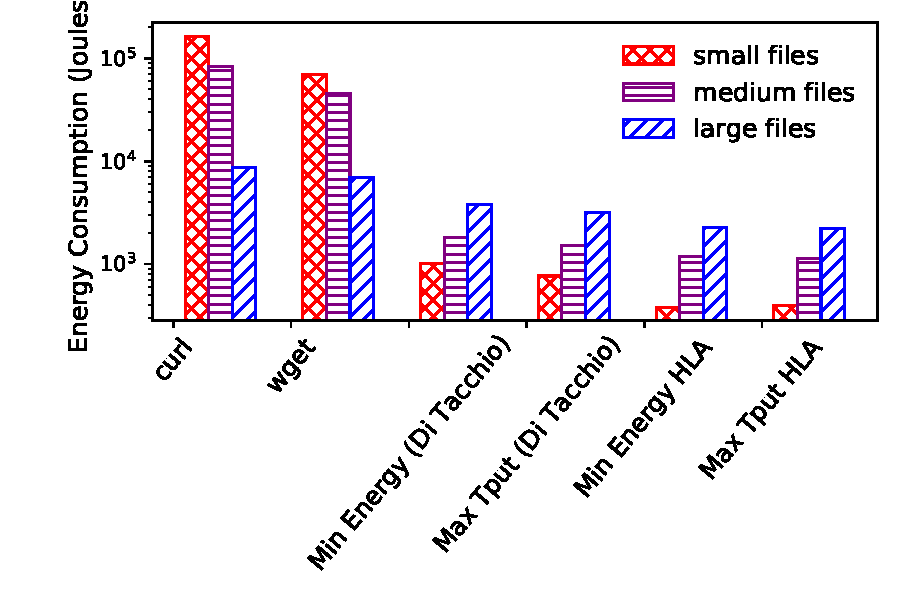
\includegraphics[width=0.47\textwidth]{images/Chameleon_Client_Energy_WGET.pdf}\par
        \hspace{5cm}
        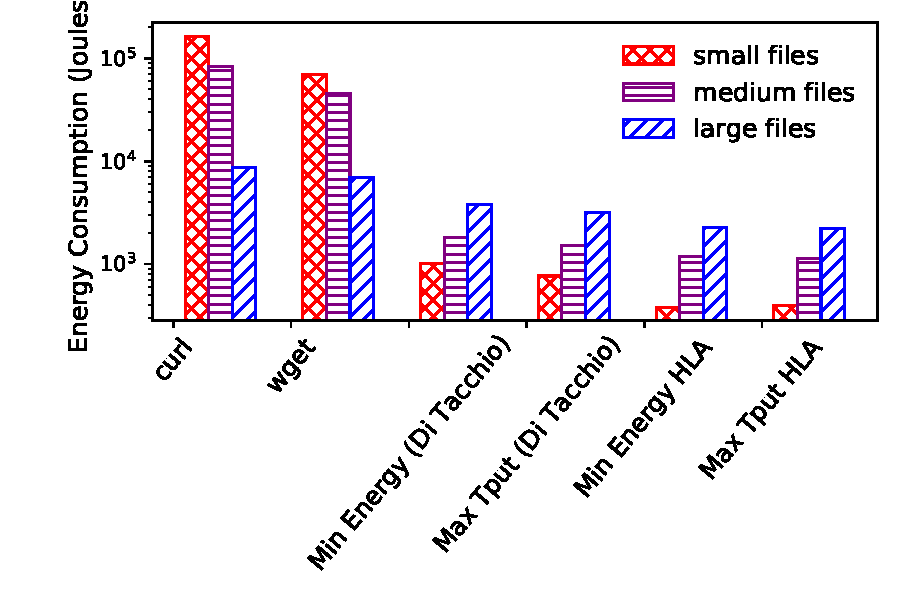
\includegraphics[width=0.47\textwidth]{images/Chameleon_Client_Energy_WGET.pdf}\par
    \end{multicols}  
    \begin{multicols}{2}
        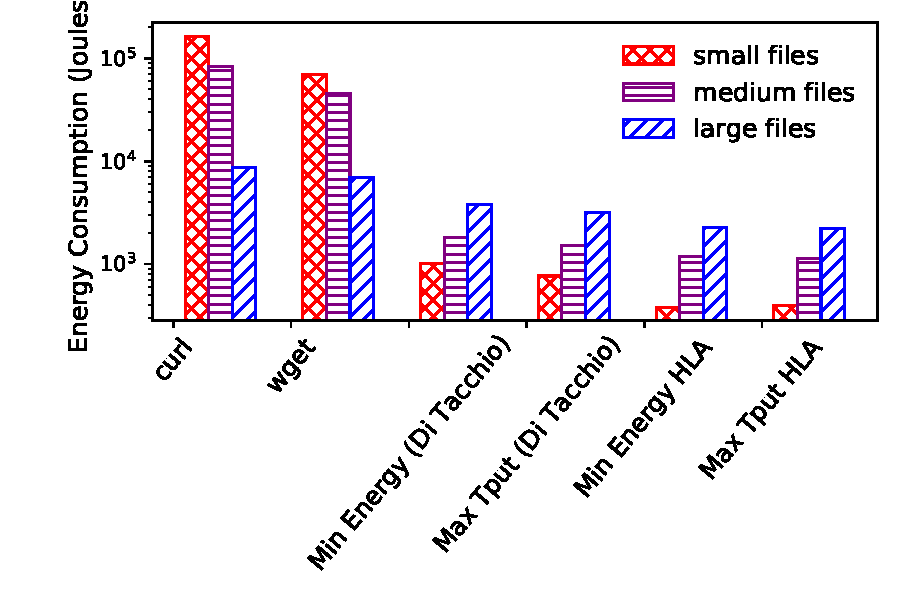
\includegraphics[width=\linewidth]{images/Chameleon_Client_Energy_WGET.pdf}\par
        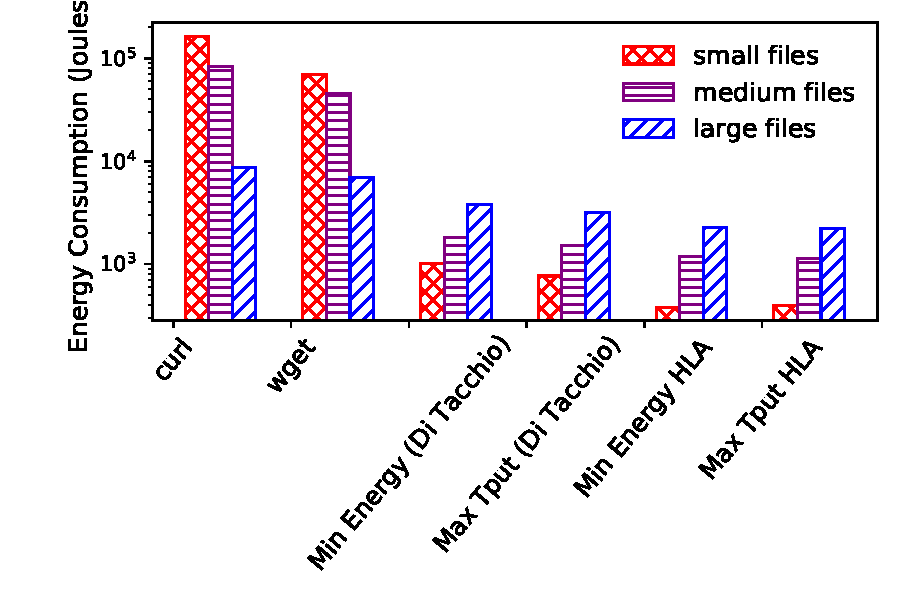
\includegraphics[width=\linewidth]{images/Chameleon_Client_Energy_WGET.pdf}\par
    \end{multicols}
    \caption{caption here}
\end{figure*}
\fi


\iffalse
\begin{figure}[t]
    \begin{centering}
	\begin{subfigure}[t]{0.9\textwidth}
    	%\centering
        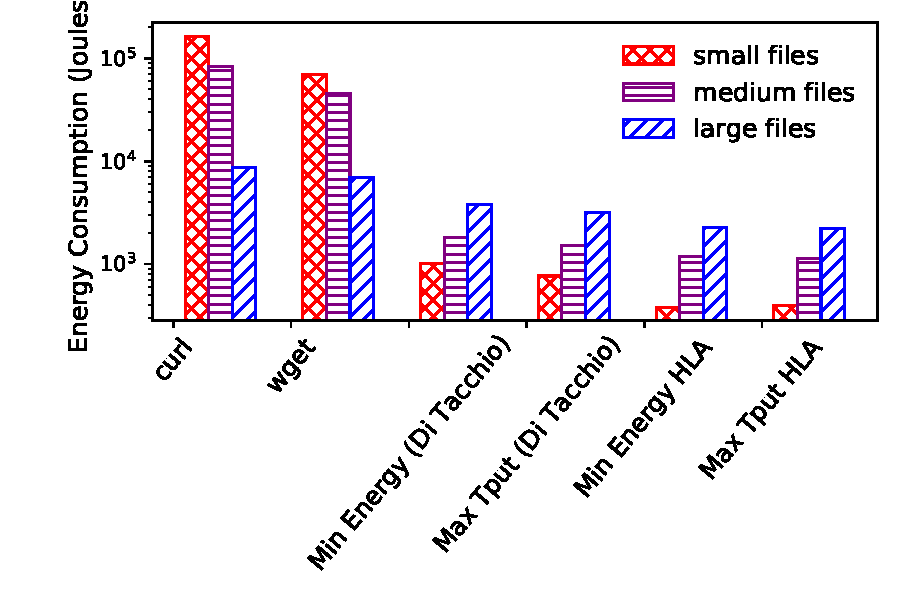
\includegraphics[keepaspectratio=true,width=75mm]{images/Chameleon_Client_Energy_WGET.pdf}
        \vspace{-2mm}
        \caption{Chameleon Cloud Client Energy consumption}
    \end{subfigure}
    \begin{subfigure}[t]{0.9\textwidth}
    	%\centering
        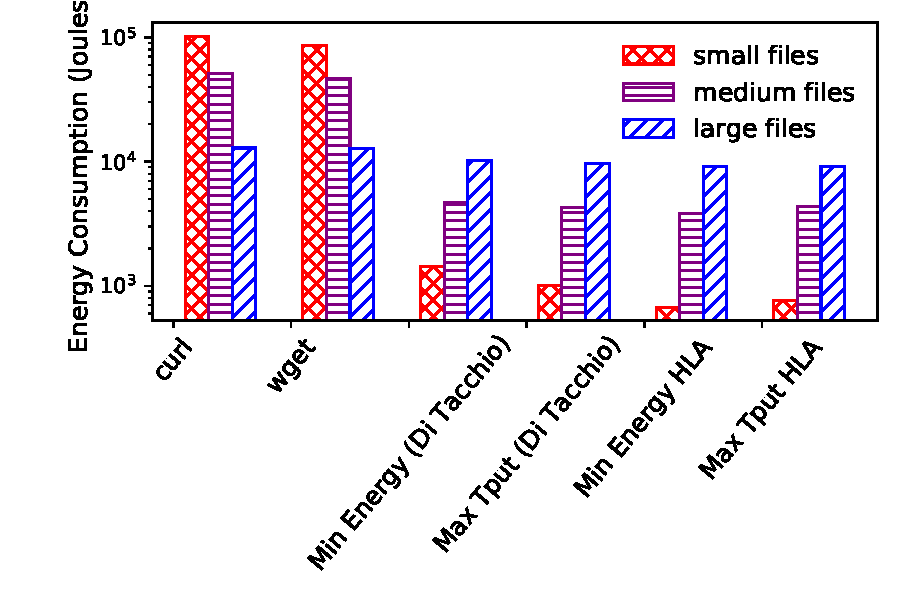
\includegraphics[keepaspectratio=true,width=50mm]{images/CloudLab_Client_Energy.pdf}
        \vspace{-2mm}
        \caption{CloudLab Client Energy Consumption}
    \end{subfigure}
    \begin{subfigure}[t]{0.2\textwidth}
    	%\centering
        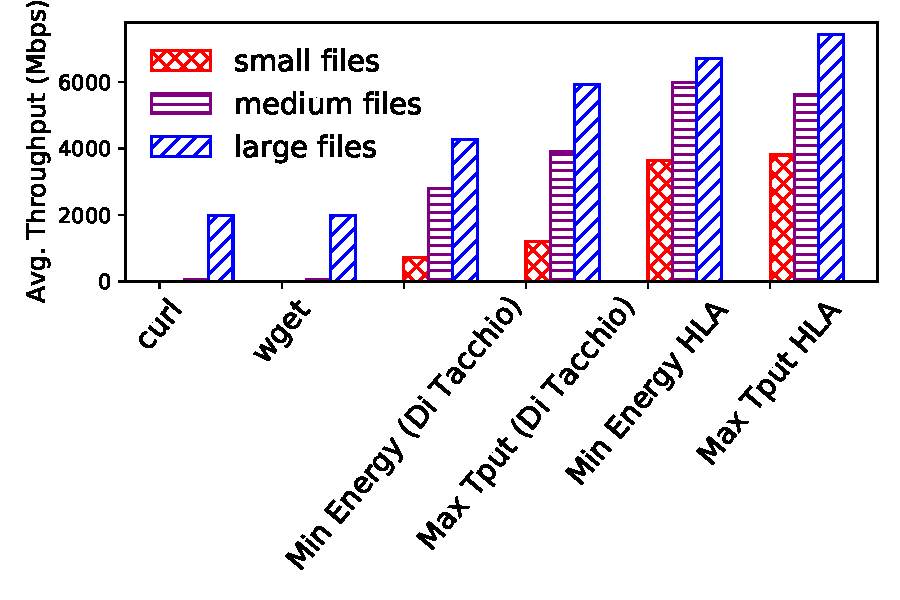
\includegraphics[keepaspectratio=true,width=45mm]{images/Chameleon_Client_Throughput.pdf}
        %\vspace{-2mm}
        \caption{Chameleon Client Avg. Throughput}
    \end{subfigure}
	\begin{subfigure}[t]{0.24\textwidth}
    	%\centering
    	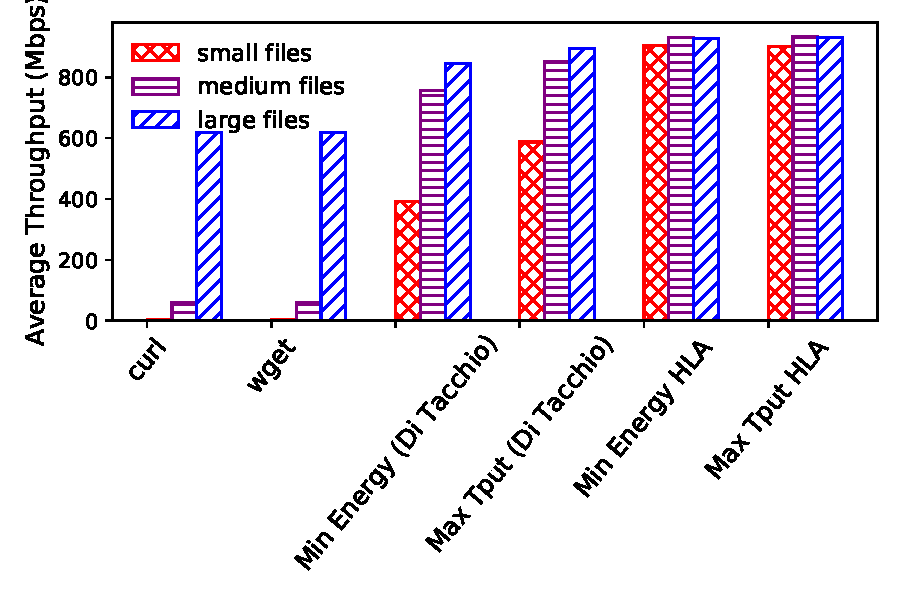
\includegraphics[keepaspectratio=true,width=45mm]{images/CloudLab_Client_Throughput.pdf}
        %\vspace{-2mm}
        \caption{CloudLab Client Avg. Throughput}
    \end{subfigure}
     \caption{Comparison of target throughput algorithms}
     \vspace{-4mm}
     \label{fig:throughputresults}
     \end{centering}
 \end{figure}
 \fi
 
 %and ii) HTTP/2, an updated version of HTTP/1.1 that multiplexes multiple application data streams over a single TCP stream to improve data transfer. \par

\iffalse %COMMENT START ********
\begin{table}[!t]
\centering
%\caption{table description}
\label{t_sim_3}
\begin{tabular}{|c|c|c|c|c|}
\hline
%\multicolumn{c}{|c|}{\textbf{Dataset}} & \multicolumn{c}{|c|}{\textbf{Num files}} & \multicolumn{c}{c|}{\textbf{Total size}} & \multicolumn{c}{c|}{\textbf{Avg file size}} & \multicolumn{c}{c|}{\textbf{Std dev}} \\ 
\textbf{Dataset} & \textbf{Num files} & \textbf{Total size} & \textbf{Avg file size} & \textbf{Std dev} \\ 
\hline
Small files & 20,000 & 1.94 GB & 101,92 KB & 29.06 KB \\  
\hline
 Medium files & 5,000 & 11.74 GB & 2.40 MB & 0.27 MB\\
\hline
Large files & 128 & 27.85 GB & 222.78 MB  & 15.19 MB \\
\hline
\end{tabular}
\caption{Characteristics of datasets}
\end{table}
\fi

 %To minimize disk activity we performed memory-to-memory data transfers. In addition, to distinguish data transfer energy from total power measurements we subtracted the baseline power consumption from the total power measurements. 
%To isolate and distinguish data transfer power consumption from total system power consumption we subtracted the system baseline power consumption from the total power readings. In addition, to mitigate the disk-to-disk and/or I/O-to-disk transfer latency, we perform memory-to-memory data transfers.
\par
%In order to compare our proposed SLA based energy efficient algorithms with Di Tacchio's energy efficient algorithms we utilized three distinct datasets.   %The mixed dataset consisting of the three aforementioned datasets. Table 2 highlights the characteristics of each dataset.

%\subsection{Comparison of minimum energy and maximum throughput algorithms}
. %However, HTTP/2 performs better due to multiplexing which decreases the number of RTTs, especially when transferring small files. However, due to a lack of parallelism and concurrency, HTTP/2 can not fully use the bandwidth.

 %On the other hand, for the Chameleon network, our energy efficient algorithms outperformed Di Tacchio’s algorithms by at least 10\% and decreased energy consumption by a minimum of 10\%. Compared to the standard data transfer tools our algorithms performed at least 20\% better and reduced energy consumption by at least 20\%. Utilizing past data transfer history as well as current network conditions our algorithms are able to converge faster to optimal parameter settings.  For the Inter-CloudLab network, which is a lower BDP network, our algorithms outperformed  Di Tacchios algorithms by at least a minimum of 5\% for all data transfers and for HTML transfers by 10\%. However, for image and video file transfers, Di Tacchio algorithms decreased energy consumption by a slightly smaller percentage which was less than 2\%; nevertheless for HTML transfers our algorithms decreased energy consumption by 10\%. For data transfers performed on the remote nodes within the cloudlab testbed,  %  why did Luigi transfer decrease energy further This is due to a slightly better concurrency estimation, or fluctuating external network consumption,  how did Zulkar say that.  but how can my throughput be better but energy consumption worser, what else could be the cause, a higher end system energy consumption, the baseline energy consumption would increase, so just find a point in the base energy that was less and use that.  and  but in the case of the. Did Luigi talk about all points 

%outperform all other algorithms in the chameleon the state-of-the-art solutions across all different scenario

%On the other hand, the algorithms proposed in this paper outperforms the state-of-the-art solutions across all different scenarios. %MinEnergyHLA reduces the energy consumption by up 5\% with respect to MinEnergy by Di Tacchio when transferring the large dataset. In addition, MaxThroughput achieves better throughput by up to 5\% and reduces/decreases the energy consumption by up to 15\% when transferring the large dataset compared to MaxThroughput by Di Tacchio. The decrease in energy consumption is due to combining offline analysis with online heuristics to better tune parameters.



%Efficiently transferring large datasets between geographically distributed locations depends on many factors, including optimal data transfer parameters such as pipelining, parallelism, and concurrency and end-system resources such as the number of CPU cores and the frequency at which they operate. Optimally tuning these five parameters during active data transfers is crucial to achieving throughput performance gains and reduced energy consumption; however, it is challenging.  

%In prior work involving predictive regression models, Yildirim et al.~\cite{yildirim2009balancing}   proposed a PCP algorithm that clustered data based on file size and performed sample transfers for each cluster. However, the sampling overhead was expensive. Yin et a. ~\cite{yin2010data} proposed a full second-order model that required at least three real-time sample transfers to find optimal parallelism levels. However, Concurrency and pipelining were not considered. Arslan et al. ~\cite{arslan2016harp} proposed predictive transfer optimization algorithms that heavily depended on heuristically initializing application-level transfer parameters to gauge network conditions. This was costly as suboptimal parameter initialization could mitigate performance gains.  

\section{Conclusion}
In this paper, we have introduced a cross-layer optimization framework that combines offline analysis with adaptive online tuning to minimize end-system energy consumption and maximize data transfer throughput performance. We presented novel algorithms that dynamically tune both application-level and kernel-level parameters based on historical log analysis and current network conditions to meet the requirements set by the service-level agreements (SLAs). Our detailed experimental analysis and results show that our proposed Cross-LayerHLA algorithms outperforms the state-of-the-art solutions in this area, reducing energy consumption considerably while increasing data transfer throughput.

\section*{Acknowledgements}
This project is in part sponsored by the National Science Foundation (NSF) under award numbers 2007829, 1724898 and 1842054. We also would like to thank the Chameleon Cloud and CloudLab for letting us use their resources in our experiments.

\bibliographystyle{IEEEtran}
\bibliography{references}
\end{document}
